%\documentclass{clases}
\documentclass[a4paper,12pt, oneside]{book}
\usepackage[skins,minted]{tcolorbox}
\usepackage[utf8]{inputenc}
\usepackage[T1]{fontenc}
\usepackage[spanish, es-tabla]{babel}
\languageshorthands{spanish}
%\usepackage{lmodern} % Usa las fuentes modernas de LaTeX
\usepackage[numbers]{natbib}
%\usepackage{morewrites}
\usepackage{inconsolata}
\usepackage{mdframed}
\usepackage{minted}
\usepackage{bm}
\usepackage{listingsutf8}
\usepackage{subcaption}
\usepackage{amsmath}
\usepackage{amssymb}
\usepackage{graphicx}
\usepackage{hyperref}
\usepackage{longtable}
\usepackage{tabularx}
\usepackage{threeparttable}
\usepackage{array}    % Necesario para centrar horizontal y verticalmente
\usepackage{xcolor}
\usepackage{pdfpages}
%\usepackage{color}
\usepackage{fancyhdr}
\usepackage{menukeys}
\usepackage{appendix}
\usepackage{fontawesome}
\usepackage{comment}
\usepackage{caption}
\usepackage{setspace}
\usepackage[explicit]{titlesec}
\usepackage{booktabs}
\usepackage[a4paper,margin=2cm]{geometry}

%\geometry{top=3cm, bottom=3cm, left=4cm, right=2cm} % Si lo quieres imprimir

\definecolor{green1}{HTML}{1dae28}
\definecolor{green2}{HTML}{afd095}
\definecolor{lightgray}{gray}{0.9}
\definecolor{orange}{RGB}{18,84,183}
\definecolor{titulo}{gray}{0.75}
\definecolor{gray97}{gray}{.97}
\definecolor{gray75}{gray}{.75}
\definecolor{gray45}{gray}{.45}
\definecolor{advertencia}{RGB}{255,178,102}
\definecolor{colorturqueza}{RGB}{178,223,238}
\definecolor{mintedbackground}{rgb}{0.95,0.95,0.95}
\definecolor{lbcolor}{rgb}{0.95,0.95,0.95}
\definecolor{mintedframe}{rgb}{0.0,0.0,0.0}
\definecolor{codebg}{rgb}{0.96,0.96,0.96}
\definecolor{colorurls}{RGB}{107,17,17}
\definecolor{colorsql}{RGB}{255,245,245}
\definecolor{colorreferences}{RGB}{48,134,3}
\definecolor{titulo}{gray}{0.65}			%------ color para fondo del titulo de tablas.

\hypersetup{
	%bookmarks=true,         % show bookmarks bar?
	unicode=true,          % non-Latin characters in Acrobat’s bookmarks
	pdftoolbar=true,        % show Acrobat’s toolbar?
	pdfmenubar=true,        % show Acrobat’s menu?
	pdffitwindow=false,     % window fit to page when opened
	pdfstartview={FitH},    % fits the width of the page to the window
	pdftitle={Reporte final de Robótica},    % title
	%	pdfauthor={},     % author
	pdfsubject={Reporte final de Robótica},   % subject of the document
	%pdfcreator={pdfTeX 3.14159265-2.6-1.40.16 (TeX Live 2016/dev)},   % creator of the document
	%pdfproducer={Panel HJ 2017}, % producer of the document
	pdfkeywords={Manipulador industrial} {Robotica} {ros} {gazebo}, % list of keywords
	%pdfnewwindow=true,      % links in new PDF window
	colorlinks=true,       % false: boxed links; true: colored links
	linkcolor=black,          % color of internal links (change box color with linkbordercolor)
	citecolor=colorreferences,        % color of links to bibliography
	filecolor=magenta,      % color of file links
	urlcolor=blue,           % color of external links
	linkbordercolor={0 0 0}
}

\lstset{
	inputencoding=utf8,
	language=Python,
	frame=Ltb,
	tabsize=2,
	framerule=0pt,
	aboveskip=0.5cm,
	framextopmargin=0pt,
	framexbottommargin=0pt,
	framexleftmargin=0.4cm,
	framesep=0pt,
	rulesep=.0pt,
	backgroundcolor=\color{gray97},
	rulesepcolor=\color{blue},
	%
	stringstyle=\ttfamily,
	showstringspaces = false,
	basicstyle=\small\ttfamily,
	commentstyle=\color{gray45},
	keywordstyle=\bfseries,
	%
	numbers=none,
	numbersep=15pt,
	numberstyle=\tiny,
	numberfirstline = false,
	breaklines=true
}

\setminted[matlab]{%
	breaklines=true,       % activa el ajuste de línea
	breakanywhere=true,    % permite partir en cualquier punto si no hay espacios
	breaksymbolleft=,      % quita el símbolo de continuación
	autogobble            % elimina sangrías comunes
%	fontsize=\footnotesize % reduce tamaño de fuente para que quepa mejor
}

\setminted[bash]{
	bgcolor=mintedbackground,
	fontfamily=tt,
	linenos=true,
	numberblanklines=true,
	numbersep=11pt,
	numbersep=2pt,
	gobble=0,
	frame=leftline,
	framesep=2mm,
	funcnamehighlighting=false,
	tabsize=4,
	obeytabs=false,
	samepage=false,
	showspaces=false,
	showtabs =false,
	texcl=false,
	baselinestretch=1.2,
	fontsize=\footnotesize,
	breaklines=true,
	breaksymbolleft=\ 
}
%\setminted{%
%	breaklines,
%	breaksymbolleft=,      % vacía la marca de continuación
%	breaksymbolright=      % también limpia el símbolo a la derecha
%}


\lstdefinestyle{consola}{
	basicstyle=\footnotesize\bf\ttfamily,
	backgroundcolor=\color{gray75},
}	
\definecolor{gray}{rgb}{0.4,0.4,0.4}
\definecolor{darkblue}{rgb}{0.0,0.0,0.6}
\definecolor{cyan}{rgb}{0.0,0.6,0.6}
\lstset{language=XML}

\lstdefinelanguage{XML}{
	morestring=[b]",
	tabsize=2,
	breaklines=true,
	morestring=[s]{>}{<},
	morecomment=[s]{<?}{?>},
	stringstyle=\color{black},
	identifierstyle=\color{darkblue},
	keywordstyle=\color{cyan},
	numbers=left,
	morekeywords={xmlns,version,type}% list your attributes here
}

\lstdefinestyle{C}{language=C}
\lstdefinestyle{XML}{language=XML}

\DeclareMathOperator{\diag}{diag}

\newtcblisting{terminal}[2][]{
	listing engine=minted,
	listing only,
	#1,
	title=#2,
	minted language=bash,
	colback=mintedbackground,
	top=0mm,
	bottom=0mm
}

\newtcblisting{matlabcode}[2][]{%
  	listing engine=minted,
	listing only,
	title=#2,
	minted language=matlab,
	minted options={%
		linenos,            % activa numeración de líneas
		numbersep=1mm,      % separación texto–números
		breaklines,         % opcional: ajuste automático
		autogobble,          % opcional: recortar sangrías
		frame=leftline,     % línea vertical a la izquierda del bloque
		framesep=1mm,
		tabsize=4,
	},
%	colback=gray!5,
%	colframe=black!70,
	top=0mm,
	bottom=0mm
	#1
}


\newtcblisting{latexcode}[2][]{%
	listing engine=minted,
	listing only,
	title=#2,
	minted language=latex,
	minted options={%
		linenos,            % activa numeración de líneas
		numbersep=1mm,      % separación texto–números
		breaklines,         % opcional: ajuste automático
		autogobble,          % opcional: recortar sangrías
		frame=leftline,     % línea vertical a la izquierda del bloque
		framesep=1mm,
		tabsize=4,
	},
	%	colback=gray!5,
	%	colframe=black!70,
	top=0mm,
	bottom=0mm
	#1
}


\newtcblisting{consolestyle}[2][]{enhanced, listing engine=minted, 
	listing only,#1, title=#2, minted language=bash, 
	coltitle=mintedbackground!35!black, 
	fonttitle=\ttfamily\footnotesize,
	sharp corners, top=0mm, bottom=0mm,
	title code={\path[draw=mintedframe, dashed, fill=mintedbackground](title.south west)--(title.south east);},
	frame code={\path[draw=mintedframe, fill=mintedbackground](frame.south west) rectangle (frame.north east);}
}

\newenvironment{doble}
{\doublespacing
}

%\newcounter{comando}[section]
%\newenvironment{comando}[1][]{\refstepcounter{comando}\par\medskip
	%	\noindent \textbf{Comando~\thecomando. #1} \rmfamily}{\medskip}
%\begin{terminal}{#1}

%\end{terminal}
%}{\medskip}

\graphicspath{{img/}{tablas/}{portada/}}  % Las imágenes se buscarán en la carpeta "img"

\addto\captionsspanish{\renewcommand{\contentsname}{Índice}}

\def\CC{{C\nolinebreak[4]\hspace{-.05em}\raisebox{.4ex}{\tiny\bf ++ \space}}}
\def\Cc{{C\nolinebreak[4]\hspace{-.05em}\raisebox{.4ex}{\tiny\bf ++}}}
\newcommand{\ffolder}[1]{\menu{\faFolderO \space #1}}
\newcommand{\ffile}[1]{\menu{\faFileO \space #1}}
\newcommand{\folder}{\faFolderO \space}
\newcommand{\file}{\faFileO \space}
\newcommand{\world}{\faGlobe \space}
\newcommand{\wworld}[1]{\menu{\faGlobe \space #1}}
\newcommand{\SB}{\{B\}} % Define el sistema del cuerpo
\newcommand{\SI}{\{I\}} % Define el sistema inercial

\newcounter{actividad} % Define un contador llamado "actividad"

\newfloat{Comando}{h}{lot}[chapter]

\renewcommand{\tablename}{Tabla}
\renewcommand{\listtablename}{Índice de tablas}
\renewcommand\listingscaption{Código}
\newcommand{\code}[1]{\colorbox{lightgray}{\texttt{#1}}}

\renewcommand\lstlistingname{Código}
\renewcommand{\appendixname}{Anexo}
\renewcommand{\appendixtocname}{Anexos}
%\renewcommand{\appendixpagename}{Anexo}
\renewcommand\labelitemi{$\bullet$}

\begin{document}
	% Aquí se encuentra el archivo con la portada
	\begin{titlepage}
	\centering
	%-------------------------------------------
	% Logos en una tabla: izquierda, centro y derecha
	\begin{tabular}{@{}p{0.3\textwidth} p{0.3\textwidth} p{0.3\textwidth}@{}}
		
\includegraphics[height=2cm]{tecnm} & 
		\centering 
\includegraphics[height=1.5cm]{SEP} & 
		\raggedleft 
\includegraphics[height=2cm]{ith.jpg} \\
	\end{tabular}
	
	\vspace{2em}
	
	\noindent
	%-------------------------------------------
	%	Información institucional y académica (esquina superior izquierda)
	\begin{minipage}[t]{0.48\textwidth}
		\raggedright
		\small \textbf{%
			Instituto Tecnológico de Hermosillo\\
			Materia: Robótica\\
			Profesor: Medina Gil Lamadrid, Jesús Iván%
		}
	\end{minipage}%
	\hfill
	%	fecha actual (esquina superior derecha), en letras pequeñas y en negrita.
	\begin{minipage}[t]{0.48\textwidth}
		\raggedleft
		\small \textbf{\today}
	\end{minipage}
	
	\vspace{2em}
	
	%-----------------------------------------
	% Unidad y Título de la tarea en letras grandes y en negrita
	{\large \textbf{Unidad 1: Morfología del robot}}\\
	{\Huge \textbf{Tipos de Sensores}}
		
	\vspace{1em}
	
	%---------------------------------------
	% Tabla con la información del equipo
	%---------------------------------------
	% Encabezado del equipo
	\begin{center}
		{\Large \textbf{Equipo 6}}
	\end{center}
	
	\vspace{1em}
	
	% Tabla de integrantes:
	% Cada fila contiene: foto (columna izquierda) y datos del integrante (columna derecha)
	\begin{center}
		\begin{tabular}{c c}
			\begin{tabular}{c}
				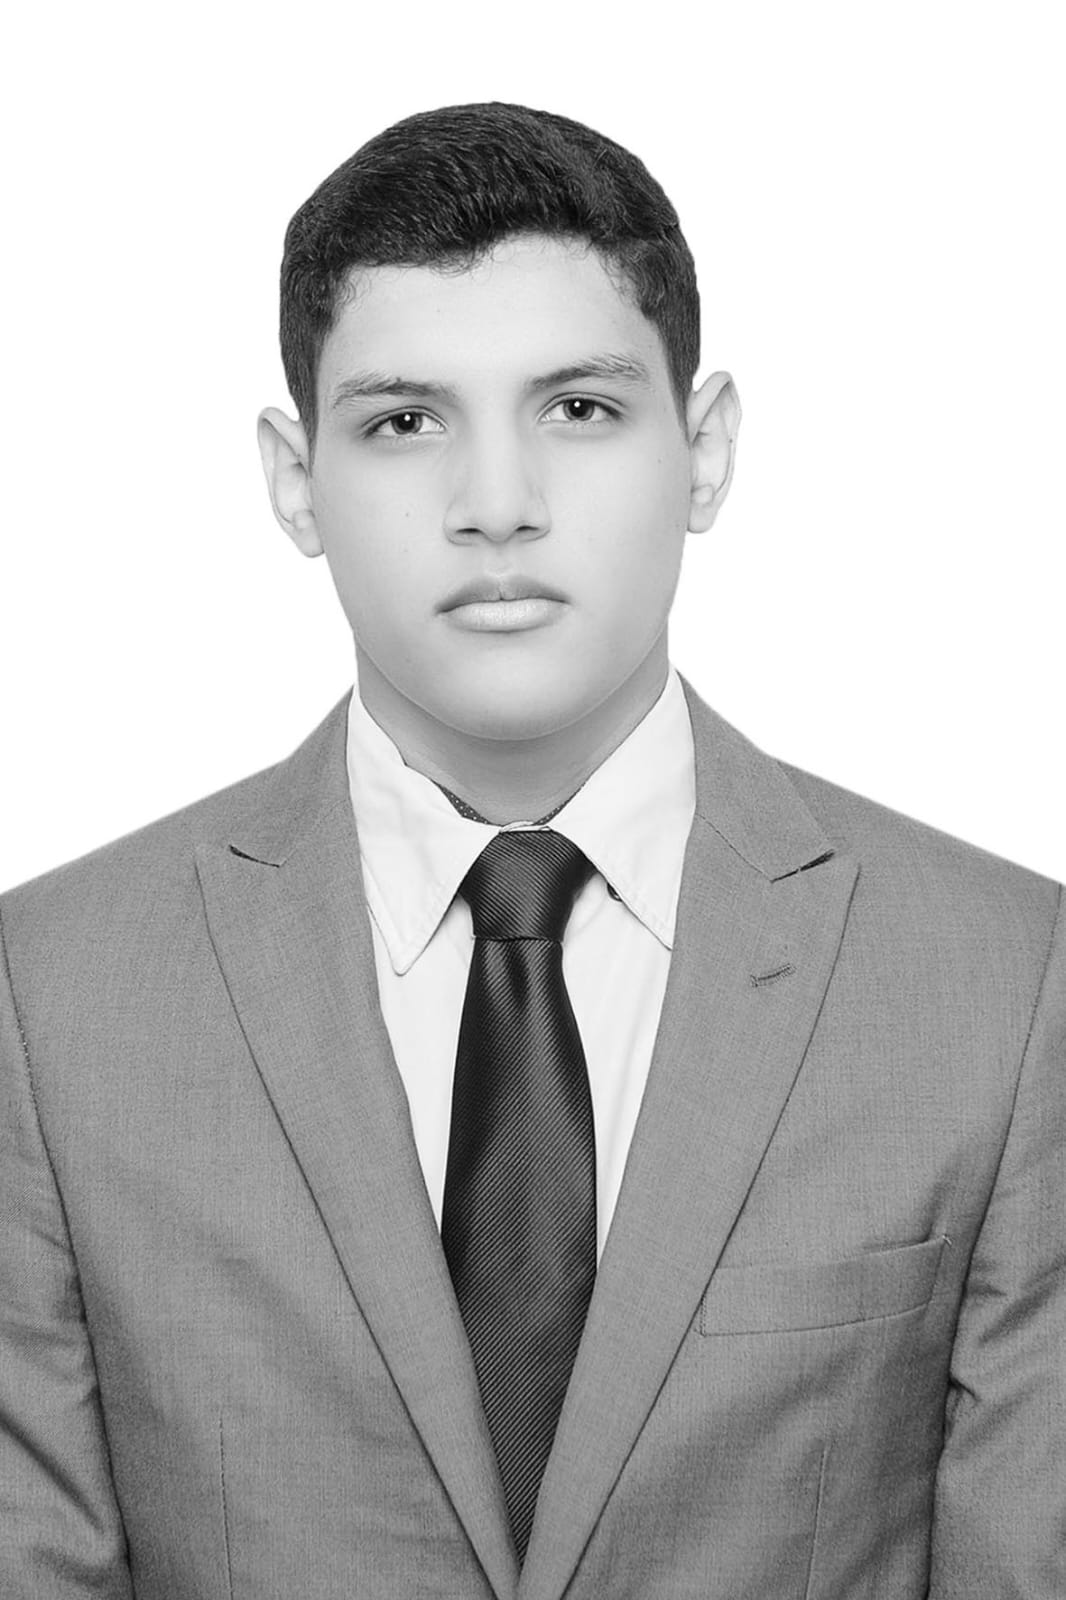
\includegraphics[height=3cm]{alexander.jpg} \\
				\textbf{Hernandez Dominguez },\\ Olinsser Alexander \\ \texttt{l21330599@hermosillo.tecnm.mx} \\ 
			\end{tabular} &
			\begin{tabular}{c}
				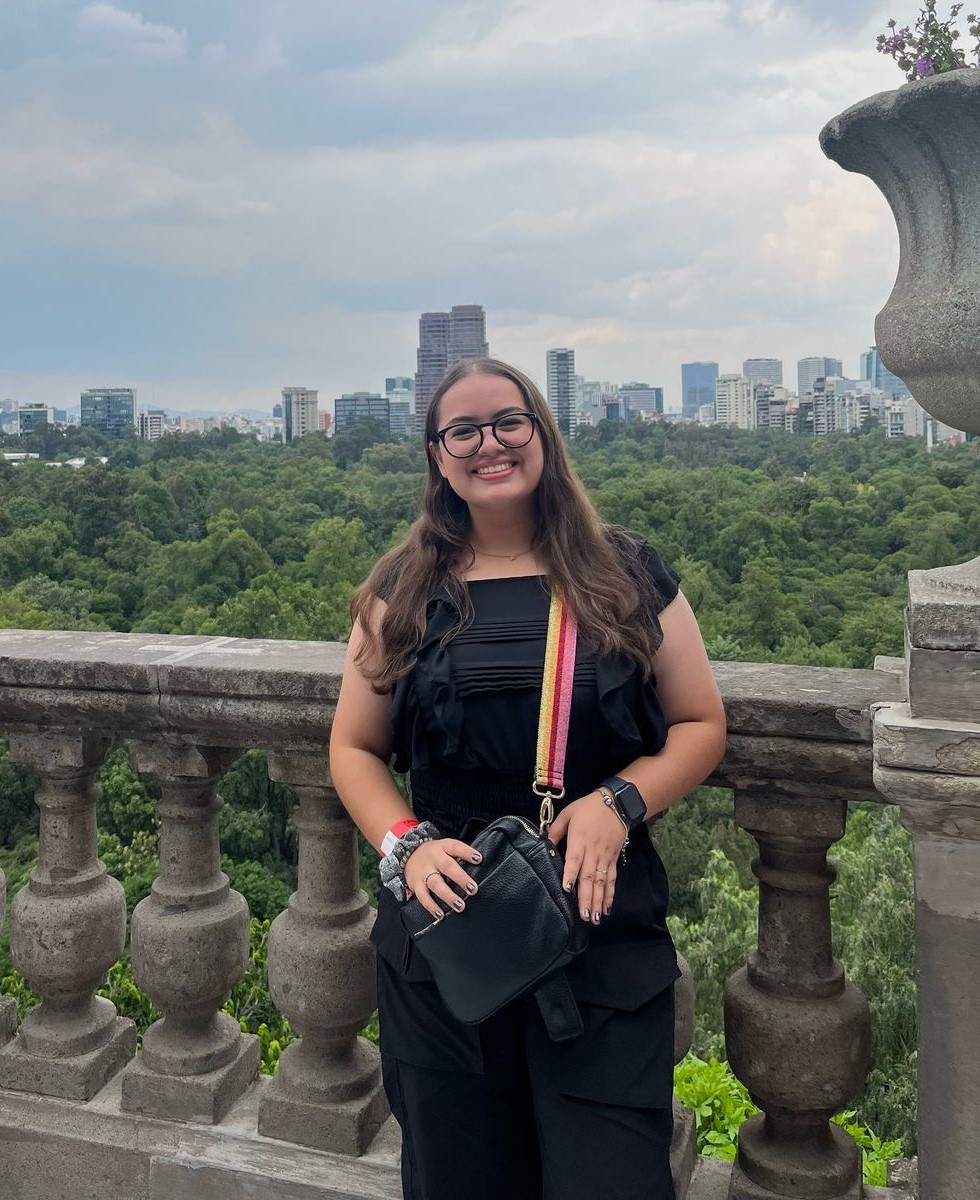
\includegraphics[height=3cm]{iliana.jpg} \\
				\textbf{Medina de la Rocha,}\\ Iliana \\ \texttt{l21330629@hermosillo.tecnm.mx} \\
			\end{tabular} \\ \vspace{2em}
			\begin{tabular}{c}
				
\includegraphics[height=3cm]{itzel.jpg} \\
				\textbf{Mesta Valdez,}\\ Itzel \\ \texttt{l21330635@hermosillo.tecnm.mx} \\ 
			\end{tabular} &
			\begin{tabular}{c}
				
\includegraphics[height=3cm]{luisa.jpg} \\
				\textbf{Santacruz López,}\\ Luisa Fernanda \\ \texttt{l21330691@hermosillo.tecnm.mx} \\ 
			\end{tabular}
		\end{tabular}
	\end{center}

\end{titlepage}

	\onehalfspacing
	\frontmatter
	\pagestyle{plain}  % numeración en páginas preliminares
	\titleformat{\chapter}
	{\bfseries\huge}
	{}
	{0pt}
	{~\raisebox{-1.5pt}{}
	\\\filleft #1 \\\vspace{.25cm}\titlerule[1.5pt]}
	
	% ---------------------------------------
	% índices
%	\clearpage   % o \cleardoublepage, según prefieras
	\newpage
	\phantomsection    % crea un nuevo destino para hyperref
	\addcontentsline{toc}{chapter}{Índice general}
	\tableofcontents
	
%	\clearpage
	\newpage
	\phantomsection
	\addcontentsline{toc}{chapter}{Índice de figuras}
	\listoffigures
	
	\hypersetup{
		linkcolor=red
	}
	
	% ---------------------------------------
	% Estilo de encabezado y pie de página
	\mainmatter
	\pagestyle{fancy}
	\fancyhead{}
	\fancyhead[L]{\leftmark}
	\fancyhead[R]{}
	\fancyfoot[L]{\parbox[l]{\textwidth-1cm}{\rightmark}}
	\fancyfoot[C]{}
	\fancyfoot[R]{\thepage}
	\renewcommand{\footrulewidth}{0.5pt}
	%\fancyfoot[RO,LE]{Diseño de modelo para simulación 3D de VANT tipo cuadricóptero}
	
	\titleformat{\chapter}
	{\bfseries\huge}
	{}
	{0pt}
	{\titlerule[3pt]~\raisebox{-1.5pt}{\sc{\chaptername}~\thechapter}~\titlerule[3pt]%
		\\\vspace{.05cm}\titlerule\\\filcenter #1 \\\vspace{.25cm}\titlerule}
	
	% Capítulo 1: Introducción
	\chapter{Introducción} \label{chap:introduccion}

El presente documento corresponde al reporte final de la materia de Robótica, en el cual se integran los conceptos y métodos abordados durante el semestre. El enfoque principal se centra en el análisis cinemático de robots manipuladores mediante el uso del método de Denavit-Hartenberg (DH), técnica ampliamente utilizada para describir la posición y orientación de eslabones y articulaciones de manera sistemática.

Como parte del desarrollo, se modeló un robot utilizando la herramienta de diseño asistido por computadora SolidWorks, al cual se le aplicaron los parámetros DH para establecer su modelo cinemático. Posteriormente, se implementó dicho modelo en el entorno de MATLAB con el objetivo de verificar y simular su comportamiento.

El reporte incluye la resolución de ejercicios específicos aplicando la metodología DH, los cuales fueron desarrollados manualmente y comprobados computacionalmente. Cada ejercicio se acompaña de representaciones gráficas, tanto esquemáticas como generadas por software, que permiten visualizar la estructura y el movimiento del robot.

Este informe tiene como finalidad demostrar la aplicación práctica de los conocimientos adquiridos, consolidando la comprensión del modelado cinemático en el contexto del diseño y análisis de sistemas robóticos.


	
	% Capítulo 2: Marco Teórico
	\chapter{Introducción} \label{chap:introduccion}

El presente documento corresponde al reporte final de la materia de Robótica, en el cual se integran los conceptos y métodos abordados durante el semestre. El enfoque principal se centra en el análisis cinemático de robots manipuladores mediante el uso del método de Denavit-Hartenberg (DH), técnica ampliamente utilizada para describir la posición y orientación de eslabones y articulaciones de manera sistemática.

Como parte del desarrollo, se modeló un robot utilizando la herramienta de diseño asistido por computadora SolidWorks, al cual se le aplicaron los parámetros DH para establecer su modelo cinemático. Posteriormente, se implementó dicho modelo en el entorno de MATLAB con el objetivo de verificar y simular su comportamiento.

El reporte incluye la resolución de ejercicios específicos aplicando la metodología DH, los cuales fueron desarrollados manualmente y comprobados computacionalmente. Cada ejercicio se acompaña de representaciones gráficas, tanto esquemáticas como generadas por software, que permiten visualizar la estructura y el movimiento del robot.

Este informe tiene como finalidad demostrar la aplicación práctica de los conocimientos adquiridos, consolidando la comprensión del modelado cinemático en el contexto del diseño y análisis de sistemas robóticos.


	
		\section{Cinemática} \label{sec:cinematica}

La cinemática es la ciencia del movimiento que estudia el movimiento sin considerar las fuerzas que lo causan. Dentro de la ciencia de la cinemática, se analizan la posición, la velocidad, la aceleración y todas las derivadas de orden superior de las variables de posición a partir de las variables articulares del sistema para analizar el comportamiento de los eslabones y articulaciones de un manipulador.
	\begin{figure}[H]
	\centering
	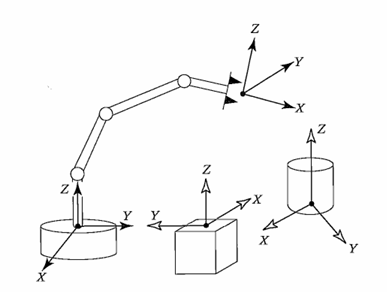
\includegraphics[width=0.7\textwidth]{img/Cinematica.png}
	\caption{Se asignan sistemas de coordenadas o 'marcos de referencia' al manipulador y a los objetos en el entorno.}
	\label{fig:Cinematica}
\end{figure}
Los manipuladores están formados por eslabones rígidos conectados mediante articulaciones que permiten el movimiento relativo entre ellos. Estas articulaciones cuentan con sensores de posición para medir dicho movimiento. En articulaciones rotatorias se habla de ángulos articulares, y en las deslizantes (prismáticas), de desplazamiento lineal o offset.

El número de grados de libertad de un manipulador indica cuántas variables independientes se necesitan para definir su posición completa. En manipuladores industriales típicos, cada articulación representa un grado de libertad, ya que son cadenas cinemáticas abiertas con articulaciones controladas individualmente.

En el extremo del manipulador se encuentra el efector final, que puede ser una herramienta específica como una pinza o un soplete. Para describir la posición del manipulador, se define un marco de coordenadas (tool frame) en el efector y otro en la base fija (base frame), y se analiza la relación entre ambos.


Para el proceso sobre cómo se llevó a cabo el algoritmo en Matlab, ir a la  \hyperref[sec:proceso_cinematica]{sección del proceso de Cinemática}.

\subsection{Cinemática Directa}

La \textbf{cinemática directa} consiste en determinar la posición y orientación del efector final del robot con base en los valores conocidos de las variables articulares. Este es el \textit{problema geométrico estático} de calcular la posición y orientación del efector final del manipulador. Específicamente, dado un conjunto de ángulos articulares, el problema de la cinemática directa consiste en calcular la posición y orientación del marco de la herramienta (\textit{tool frame}) con respecto al marco base (\textit{base frame}). A veces, se considera este proceso como un \textit{cambio de representación} de la posición del manipulador, pasando de una descripción en el \textit{espacio articular} a una descripción en el espacio cartesiano.

Para resolver este problema, se utiliza comúnmente el \textbf{método de Denavit-Hartenberg (DH)}, una convención estandarizada que permite representar de forma sistemática la geometría de un manipulador robótico. Este método simplifica el proceso de modelado mediante la asignación de un sistema de coordenadas a cada eslabón del robot y la definición de las transformaciones relativas entre eslabones consecutivos utilizando solo cuatro parámetros:

\begin{itemize}
	\item $\theta$: ángulo de rotación alrededor del eje $z$ (variable para articulaciones rotacionales).
	\item $d$: desplazamiento a lo largo del eje $z$ (variable para articulaciones prismáticas).
	\item $a$: longitud del eslabón, medida a lo largo del eje $x$.
	\item $\alpha$: ángulo de torsión, es decir, la rotación alrededor del eje $x$ entre dos ejes $z$ consecutivos.
\end{itemize}

La formulación de Denavit-Hartenberg permite obtener una matriz de transformación homogénea $4 \times 4$ para cada par de eslabones, que incorpora rotaciones y traslaciones en el espacio tridimensional. Al multiplicar secuencialmente estas matrices desde el eslabón base hasta el efector final, se obtiene una única matriz que describe completamente la postura del robot, es decir, la posición y orientación del efector con respecto al sistema de referencia global.

Una de las principales ventajas del método DH es su capacidad para estandarizar el modelado de robots con diferentes configuraciones geométricas, lo que facilita la implementación computacional y la interpretación de resultados. En este proyecto, los parámetros DH fueron determinados a partir del modelo CAD del robot desarrollado en SolidWorks, y posteriormente implementados en \texttt{MATLAB} para calcular las matrices de transformación y verificar los resultados mediante simulación gráfica.

\subsection{Cinemática Diferencial}
La \textbf{cinemática diferencial} se encarga de analizar cómo las velocidades articulares afectan la velocidad lineal y angular del efector final de un manipulador robótico. Este análisis es fundamental para el diseño de sistemas de control y planificación de trayectorias en robótica.

\subsubsection{El Jacobiano}

El \textbf{Jacobiano} es una matriz que relaciona las velocidades articulares del robot con las velocidades lineales y angulares del efector final. Matemáticamente, se expresa como:

\[
\dot{\mathbf{x}} = \mathbf{J}(\mathbf{q}) \, \dot{\mathbf{q}}
\]

donde:
\begin{itemize}
	\item $\dot{\mathbf{x}}$ es el vector de velocidades del efector final (lineales y angulares).
	\item $\mathbf{J}(\mathbf{q})$ es la matriz Jacobiana, que depende de las coordenadas articulares $\mathbf{q}$.
	\item $\dot{\mathbf{q}}$ es el vector de velocidades articulares.
\end{itemize}

Cada columna de la matriz Jacobiana representa la contribución de una articulación individual a la velocidad del efector final. Por ejemplo, en un manipulador con $n$ grados de libertad, la $i$-ésima columna de $\mathbf{J}$ describe el efecto de la velocidad de la articulación $i$ en la velocidad del efector final, considerando que las demás articulaciones están fijas.
	\begin{figure}[H]
	\centering
	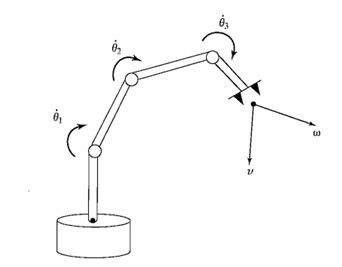
\includegraphics[width=0.7\textwidth]{img/jacobiano.png}
	\caption{La relación geométrica entre las velocidades articulares y la velocidad del efector final puede describirse mediante una matriz llamada Jacobiana.}
	\label{fig:Jacobiano}
\end{figure}

\subsubsection{Aplicaciones del Jacobiano}

El Jacobiano tiene múltiples aplicaciones en robótica, entre las que se incluyen:
\begin{itemize}
	\item \textbf{Análisis de singularidades}: Determinar configuraciones en las que el manipulador pierde grados de libertad o se vuelve incapaz de moverse en ciertas direcciones.
	\item \textbf{Control de velocidad}: Calcular las velocidades articulares necesarias para lograr una velocidad deseada del efector final.
	\item \textbf{Dinámica inversa}: Relacionar fuerzas y torques en el efector final con las fuerzas y torques en las articulaciones.
\end{itemize}

\subsubsection{Cálculo del Jacobiano}

El cálculo de la matriz Jacobiana puede realizarse utilizando métodos analíticos o numéricos. En este proyecto, se empleó el método analítico, derivando las expresiones de las posiciones del efector final con respecto a las coordenadas articulares y calculando las derivadas parciales correspondientes.

\subsubsection{Ejemplo de Jacobiano para una Articulación Rotacional}

Para una articulación rotacional, la contribución a la velocidad lineal del efector final se puede calcular como:

\[
\mathbf{v}_i = \mathbf{z}_{i-1} \times (\mathbf{o}_n - \mathbf{o}_{i-1})
\]

y la contribución a la velocidad angular es:

\[
\boldsymbol{\omega}_i = \mathbf{z}_{i-1}
\]

donde:
\begin{itemize}
	\item $\mathbf{z}_{i-1}$ es el eje de rotación de la articulación $i$ en el marco de referencia base.
	\item $\mathbf{o}_n$ es el vector de posición del efector final.
	\item $\mathbf{o}_{i-1}$ es el vector de posición de la articulación $i$.
\end{itemize}

Estas expresiones se utilizan para construir las columnas correspondientes de la matriz Jacobiana.

\subsubsection{Implementación en MATLAB}

En el presente proyecto, se implementó el cálculo del Jacobiano en \texttt{MATLAB}, utilizando las expresiones analíticas derivadas y verificando los resultados mediante simulaciones. Esta implementación permitió analizar el comportamiento del manipulador en diferentes configuraciones y validar la precisión del modelo cinemático.



\subsection{Cinemática Inversa}

La \textbf{cinemática inversa} es el proceso mediante el cual se determinan los valores articulares necesarios para que el efector final de un robot manipulador alcance una posición y orientación deseadas en el espacio cartesiano tridimensional. En otras palabras, dado un objetivo en términos de coordenadas y orientación en el espacio, el objetivo de la cinemática inversa es encontrar todos los posibles conjuntos de variables articulares que produzcan esa configuración final.

	\begin{figure}[H]
	\centering
	\includegraphics[width=0.7\textwidth]{img/cinematicainv.png}
	\caption{Para una posición y orientación dadas del marco de la herramienta, los valores de las variables articulares pueden calcularse mediante la cinemática inversa.}
	\label{fig:CinematicaInversa}
\end{figure}

Este problema es fundamental en la programación de manipuladores robóticos, ya que las trayectorias y tareas generalmente se especifican en el espacio cartesiano, mientras que el movimiento del robot se controla en su espacio articular. Por lo tanto, es necesario disponer de algoritmos que realicen la conversión entre ambos espacios.

A diferencia de la cinemática directa, las ecuaciones que definen la cinemática inversa son no lineales y, por lo tanto, pueden presentar múltiples soluciones o no tener ninguna, dependiendo de si el punto deseado se encuentra dentro del \textit{espacio de trabajo} del manipulador. Esta complejidad hace que, en muchos casos, no se pueda obtener una solución analítica cerrada, y se deban utilizar métodos numéricos o aproximados.

Uno de los enfoques numéricos más comunes es el uso de algoritmos basados en el \textbf{gradiente del error} y el \textbf{jacobiano}. El jacobiano $\mathbf{J}(\mathbf{q})$ describe la relación entre las velocidades articulares $\dot{\mathbf{q}}$ y las velocidades del efector final $\dot{\mathbf{x}}$ mediante la ecuación:

\[
\dot{\mathbf{x}} = \mathbf{J}(\mathbf{q}) \, \dot{\mathbf{q}}
\]

Este mismo jacobiano se puede utilizar para propagar pequeños cambios en la posición del efector final hacia ajustes en los valores articulares. El \textbf{gradiente del error} entre la posición deseada y la actual se proyecta en el espacio articular mediante el jacobiano transpuesto o su pseudo-inversa, dependiendo del método seleccionado.

Cabe destacar que existen múltiples métodos para resolver el problema de la cinemática inversa, incluyendo:
\subsubsection{Métodos para la Resolución de la Cinemática Inversa}

Existen diversos enfoques para resolver el problema de la cinemática inversa. A continuación, se describen los principales métodos empleados, junto con sus características, ventajas y limitaciones.

\paragraph{1. Métodos Geométricos}

Estos métodos se basan en el análisis de la geometría del robot, utilizando relaciones trigonométricas simples (como la ley de senos y cosenos) para calcular directamente los ángulos articulares.

\begin{itemize}
	\item \textbf{Ventajas:} Rápidos y computacionalmente eficientes. Pueden ofrecer soluciones analíticas cerradas.
	\item \textbf{Limitaciones:} Solo aplicables a robots con geometría sencilla (como robots planos o tipo SCARA).
	\item \textbf{Ejemplo de uso:} Cálculo de ángulos para un manipulador plano de 2 grados de libertad (2-DOF).
\end{itemize}

\paragraph{2. Métodos Algebraicos}

Consisten en plantear y resolver sistemas de ecuaciones no lineales que relacionan las coordenadas del efector final con las variables articulares.

\begin{itemize}
	\item \textbf{Ventajas:} Posibilidad de obtener soluciones exactas si el sistema es resoluble.
	\item \textbf{Limitaciones:} Las ecuaciones pueden ser complejas o no tener solución cerrada, especialmente en manipuladores con múltiples grados de libertad.
	\item \textbf{Ejemplo de uso:} Resolución simbólica de la cinemática inversa de un robot tipo PUMA.
\end{itemize}

\paragraph{3. Métodos Numéricos Iterativos}

Estos métodos aproximan las soluciones mediante iteraciones sucesivas, partiendo de una configuración inicial y ajustando las variables articulares en función del error entre la posición actual y la deseada.

\begin{itemize}
	\item \textbf{Ventajas:} Generalizables a robots complejos. No requieren una solución cerrada.
	\item \textbf{Limitaciones:} Pueden no converger o ser sensibles a la elección del punto inicial.
\end{itemize}

Los principales métodos iterativos son:

\begin{itemize}
	\item \textbf{a) Método del Jacobiano Transpuesto:}
	
	\[
	\Delta \mathbf{q} = \alpha \, \mathbf{J}^T(\mathbf{q}) \, (\mathbf{x}_d - \mathbf{x})
	\]
	
	Utiliza el jacobiano transpuesto para proyectar el error cartesiano al espacio articular. Es simple y efectivo para tareas básicas.
	
	\item \textbf{b) Método de la Pseudo-inversa del Jacobiano:}
	
	\[
	\Delta \mathbf{q} = \mathbf{J}^+(\mathbf{q}) \, (\mathbf{x}_d - \mathbf{x})
	\]
	
	Usa la pseudo-inversa de Moore-Penrose y es adecuado para robots redundantes. Minimiza el error cartesiano de forma más precisa.
	
	\item \textbf{c) Método de Newton-Raphson:}
	
	\[
	\mathbf{q}_{k+1} = \mathbf{q}_k + \mathbf{J}^+(\mathbf{q}_k) \cdot (\mathbf{x}_d - f(\mathbf{q}_k))
	\]
	
	Se basa en una aproximación derivativa para encontrar rápidamente una solución, siempre que se inicie desde una configuración cercana a la correcta.
	
	\item \textbf{d) Método del Gradiente Descendente:}
	
	\[
	E(\mathbf{q}) = \frac{1}{2} \| \mathbf{x}_d - f(\mathbf{q}) \|^2, \quad \mathbf{q}_{k+1} = \mathbf{q}_k - \eta \nabla E(\mathbf{q}_k)
	\]
	
	Minimiza directamente la función de error entre la posición deseada y la alcanzada. Es robusto, pero converge lentamente.
\end{itemize}

\paragraph{4. Comparación de Métodos}

\begin{table}[H]
	\centering
	\begin{tabular}{|l|c|c|c|c|}
		\hline
		\textbf{Método} & \textbf{Precisión} & \textbf{Rapidez} & \textbf{Robustez} & \textbf{Aplicabilidad} \\
		\hline
		Geométrico & Alta & Alta & Media & Robots simples \\
		Algebraico & Alta & Media & Media & Robots con solución cerrada \\
		Jacobiano Transpuesto & Media & Alta & Media & Robots generales \\
		Pseudo-inversa & Alta & Media & Media & Robots redundantes \\
		Newton-Raphson & Alta & Alta & Baja & Estimación inicial cercana \\
		Gradiente Descendente & Media & Baja & Alta & Evitación de obstáculos \\
		\hline
	\end{tabular}
	\caption{Comparación de métodos de resolución de cinemática inversa}
\end{table}


En este proyecto, se implementó un método iterativo basado en el uso del jacobiano y el gradiente del error para aproximar las configuraciones articulares que permiten al efector final alcanzar una posición deseada. Este enfoque es especialmente útil para robots con múltiples grados de libertad o geometrías complejas, donde los métodos analíticos no son factibles.

El estudio de la cinemática inversa permite comprender los límites y capacidades del robot en cuanto a su movilidad, así como diseñar algoritmos de control y planificación de movimientos más eficientes.



		
		\section{ROS} \label{sec:ros}

\begin{figure}[h]
	\centering
	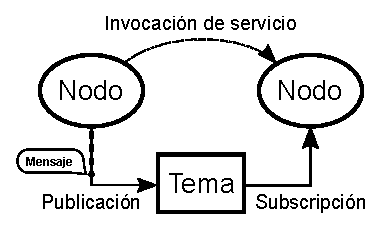
\includegraphics[width=0.5\linewidth]{img/ROS_concepts}
	\caption{Diagrama de comunicación de ROS}
	\label{fig:rosconcepts}
\end{figure}

El \textbf{Robot Operating System (ROS)} es un conjunto de bibliotecas y herramientas de software de código abierto que facilitan el desarrollo de aplicaciones robóticas. Aunque su nombre sugiere que es un sistema operativo, en realidad, ROS actúa como un \textit{middleware} que proporciona servicios similares a los de un sistema operativo, tales como abstracción de hardware, control de dispositivos de bajo nivel, implementación de funcionalidades comunes, paso de mensajes entre procesos y gestión de paquetes. 

\subsubsection*{Características principales de ROS}

\begin{itemize}
	\item \textbf{Abstracción de hardware}: Permite a los desarrolladores interactuar con diferentes componentes de hardware sin preocuparse por las especificaciones particulares de cada dispositivo.
	\item \textbf{Sistema de mensajes}: Facilita la comunicación entre procesos mediante un sistema de paso de mensajes, lo que permite que diferentes nodos (procesos) intercambien información de manera eficiente.
	\item \textbf{Gestión de paquetes}: ROS organiza el software en paquetes, cada uno de los cuales puede contener bibliotecas, ejecutables, scripts y otros recursos necesarios para una funcionalidad específica.
	\item \textbf{Herramientas de desarrollo}: Incluye herramientas para visualizar datos, depurar aplicaciones y gestionar la ejecución de múltiples nodos.
\end{itemize}

\subsubsection*{Estructura de ROS}

ROS se basa en una arquitectura de grafo de computación, donde los nodos representan procesos que realizan tareas específicas y se comunican entre sí mediante temas (\textit{topics}), servicios (\textit{services}) y acciones (\textit{actions}). Esta estructura modular permite desarrollar sistemas robóticos complejos de manera escalable y flexible \cite{ros_wiki_concepts}.

\subsubsection*{Versiones de ROS}

Existen dos versiones principales de ROS:

\begin{itemize}
	\item \textbf{ROS 1}: La versión original, ampliamente utilizada en la comunidad robótica. Proporciona una amplia gama de paquetes y herramientas para diversas aplicaciones.
	\item \textbf{ROS 2}: Una reescritura de ROS 1 que aborda limitaciones anteriores, ofreciendo mejoras en términos de seguridad, rendimiento en tiempo real y soporte para sistemas distribuidos. La última versión LTS es \textit{Jazzy Jalisco}, lanzada en mayo de 2024 \cite{ros_home}.
\end{itemize}

\subsubsection{Aplicaciones de ROS}

ROS se utiliza en una amplia variedad de aplicaciones robóticas, incluyendo:

\begin{itemize}
	\item \textbf{Robots móviles}: Para navegación, mapeo y evitación de obstáculos.
	\item \textbf{Manipuladores robóticos}: En tareas de control de brazos robóticos y pinzas.
	\item \textbf{Robótica industrial}: A través de iniciativas como ROS-Industrial, que extiende las capacidades de ROS al ámbito de la automatización industrial \cite{ros_industrial}.
	\item \textbf{Investigación y educación}: Como plataforma estándar para el desarrollo y enseñanza de conceptos robóticos.
\end{itemize}

\subsubsection{Recursos y comunidad}

ROS cuenta con una comunidad activa y una amplia documentación disponible en línea. Los recursos incluyen:

\begin{itemize}
	\item \textbf{Sitio oficial}: \url{https://www.ros.org/}
	\item \textbf{Wiki de ROS}: \url{https://wiki.ros.org/}
	\item \textbf{Foros de discusión}: \url{https://discourse.ros.org/}
	\item \textbf{Repositorio de paquetes}: \url{https://index.ros.org/}
\end{itemize}

\subsection{Nodo (Node)}
\subsection{Tema (Topic)}
\subsection{Mensaje (Message)}
\subsection{Servicio (Service)}
\subsection{Gazebo}
\subsection{RViz}

		
		\section{Dinámica} \label{sec:dinamica}

La dinámica de robots se encarga del estudio de cómo las fuerzas y torques afectan el movimiento de un robot. A diferencia de la cinemática, que sólo considera posiciones, velocidades y aceleraciones, la dinámica incluye también las **fuerzas** que causan dichos movimientos.

El modelo dinámico de un robot manipulador se representa generalmente en coordenadas articulares \( \mathbf{q} \), e incluye la interacción entre masa, inercia, efectos centrífugos y de Coriolis, gravedad, fricción y perturbaciones externas. El modelo completo tiene la forma:

\begin{equation}
	\mathbf{M}(\mathbf{q})\ddot{\mathbf{q}} + \mathbf{C}(\mathbf{q}, \dot{\mathbf{q}})\dot{\mathbf{q}} + \mathbf{g}(\mathbf{q}) = \boldsymbol{\tau}
\end{equation}

Donde:

\begin{itemize}
	\item \( \mathbf{q} \): Vector de coordenadas articulares (por ejemplo, ángulos o desplazamientos).
	\item \( \ddot{\mathbf{q}} \): Aceleraciones articulares.
	\item \( \mathbf{M}(\mathbf{q}) \): Matriz de inercia o masa generalizada.
	\item \( \mathbf{C}(\mathbf{q}, \dot{\mathbf{q}}) \): Términos centrífugos y de Coriolis.
	\item \( \mathbf{g}(\mathbf{q}) \): Vector de torques debido a la gravedad.
	\item \( \boldsymbol{\tau} \): Vector de torques aplicados por los actuadores.
\end{itemize}

\subsubsection{Matriz de masa o inercia \( \mathbf{M}(\mathbf{q}) \)}

La matriz de masa describe la inercia del sistema con respecto a sus coordenadas articulares. Depende de la masa y la distribución de masa (es decir, los tensores de inercia) de cada eslabón del robot. Se obtiene a partir de la energía cinética del sistema:

\begin{equation}
	E_c = \frac{1}{2} \sum_{i=1}^{n} m_i \mathbf{v}_i^T \mathbf{v}_i + \frac{1}{2} \sum_{i=1}^{n} \boldsymbol{\omega}_i^T \mathbf{J}_i \boldsymbol{\omega}_i
\end{equation}

Donde:

\begin{itemize}
	\item \( m_i \): Masa del eslabón \( i \).
	\item \( \mathbf{v}_i \): Velocidad lineal del centro de masa del eslabón \( i \).
	\item \( \boldsymbol{\omega}_i \): Velocidad angular del eslabón \( i \).
	\item \( \mathbf{J}_i \): Tensor de inercia del eslabón \( i \) respecto a su centro de masa.
\end{itemize}

Esta matriz es simétrica y definida positiva, lo que garantiza estabilidad física.

\subsubsection{Términos de Coriolis y centrífugos \( \mathbf{C}(\mathbf{q}, \dot{\mathbf{q}}) \)}

Cuando un robot está en movimiento, aparecen fuerzas adicionales debido a la interacción entre las velocidades de las articulaciones. Estas fuerzas se dividen en:

\begin{itemize}
	\item \textbf{Fuerzas centrífugas:} Proporcionales al cuadrado de la velocidad.
	\item \textbf{Fuerzas de Coriolis:} Proporcionales al producto cruzado entre velocidades.
\end{itemize}

Estas fuerzas se agrupan en la matriz \( \mathbf{C}(\mathbf{q}, \dot{\mathbf{q}}) \), que puede derivarse a partir de la matriz de inercia usando:

\begin{equation}
	C_{ijk} = \frac{1}{2} \left( \frac{\partial M_{ij}}{\partial q_k} + \frac{\partial M_{ik}}{\partial q_j} - \frac{\partial M_{jk}}{\partial q_i} \right)
\end{equation}

\subsubsection{Vector de gravedad \( \mathbf{g}(\mathbf{q}) \)}

El peso de cada eslabón genera torques en las articulaciones dependiendo de la configuración del robot. Estas fuerzas se agrupan en el vector \( \mathbf{g}(\mathbf{q}) \), y su forma general es:

\begin{equation}
	\mathbf{g}(\mathbf{q}) = \sum_{i=1}^{n} m_i g \frac{\partial h_i}{\partial \mathbf{q}}
\end{equation}

Donde \( h_i \) es la altura del centro de masa del eslabón \( i \) en el sistema de coordenadas global. Este término es fundamental para realizar compensación de gravedad en controladores de robots.

\subsubsection{Fricción}

La fricción es un efecto no conservativo que se opone al movimiento y depende de la velocidad de las articulaciones. Se considera de dos tipos:

\begin{itemize}
	\item \textbf{Fricción estática:} Torque necesario para iniciar el movimiento.
	\item \textbf{Fricción viscosa:} Proporcional a la velocidad articular.
\end{itemize}

El modelo combinado puede expresarse como:

\begin{equation}
	\tau_{\text{fricción}} = K_v \dot{q} + \tau_s \cdot \text{sign}(\dot{q})
\end{equation}

donde \( K_v \) es el coeficiente de fricción viscosa y \( \tau_s \) es el torque de fricción estática.

\subsubsection{Perturbaciones externas}

Finalmente, el robot puede estar sujeto a fuerzas externas no modeladas, como colisiones, fuerzas del entorno o errores de calibración. Estas se incluyen como un torque perturbador \( \tau_{\text{perturbador}} \) que se resta del torque total aplicado:

\begin{equation}
	\boldsymbol{\tau}_{\text{total}} = \boldsymbol{\tau}_{\text{motor}} - \boldsymbol{\tau}_{\text{perturbador}} - \boldsymbol{\tau}_{\text{fricción}}
\end{equation}

Estas perturbaciones son relevantes en aplicaciones donde el entorno no es completamente conocido o en robótica colaborativa donde hay contacto humano-robot.

		
		\section{Control} \label{sec:control}
Algún día lograré explicar bien el Control de su robot, pero este semestre no será supongo. Así que pueden comentar el input de esta parte, pero igual pueden intentar explicar esto.


	
	% Capítulo 3: Desarrollo
	\chapter{Introducción} \label{chap:introduccion}

El presente documento corresponde al reporte final de la materia de Robótica, en el cual se integran los conceptos y métodos abordados durante el semestre. El enfoque principal se centra en el análisis cinemático de robots manipuladores mediante el uso del método de Denavit-Hartenberg (DH), técnica ampliamente utilizada para describir la posición y orientación de eslabones y articulaciones de manera sistemática.

Como parte del desarrollo, se modeló un robot utilizando la herramienta de diseño asistido por computadora SolidWorks, al cual se le aplicaron los parámetros DH para establecer su modelo cinemático. Posteriormente, se implementó dicho modelo en el entorno de MATLAB con el objetivo de verificar y simular su comportamiento.

El reporte incluye la resolución de ejercicios específicos aplicando la metodología DH, los cuales fueron desarrollados manualmente y comprobados computacionalmente. Cada ejercicio se acompaña de representaciones gráficas, tanto esquemáticas como generadas por software, que permiten visualizar la estructura y el movimiento del robot.

Este informe tiene como finalidad demostrar la aplicación práctica de los conocimientos adquiridos, consolidando la comprensión del modelado cinemático en el contexto del diseño y análisis de sistemas robóticos.


	
		\section{Características del Robot} \label{sec:caracteristicas_del_robot}

\begin{table}[ht]
	\centering
	\caption{Parámetros de Denavit Hartenberg y límites del robot}
	\label{tab:parametros_robot}
	\begin{tabular}{l|ccccccccc}
		\toprule
		N & {$\theta$} & {$d$} & {$a$} & {$\alpha$} & {tipo} 
		& {$q_{\min}$} & {$q_{\max}$} 
		& {$\dot q_{\max}$} & {$\ddot q_{\max}$} \\
		\midrule
		1 & 0   & 496.00 & 0   & 90 & r & -180 & 180 & 180 & 360 \\
		2 & 90  & 0.00   & 500 & 0  & r & -90  & 90  & 180 & 360 \\
		3 & 90  & 451.38 & 0   & 90 & r & -180 & 0   & 180 & 360 \\
		4 & 90  & 195.00 & 0   & 90 & r & -180 & 0   & 180 & 360 \\
		\bottomrule
	\end{tabular}
\end{table}

\bigskip
\noindent
\textbf{Donde:}
\begin{description}
	\item[N] Número de la articulación.
	\item[\(\theta\)] Ángulo articular (grados).
	\item[\(d\)] Desplazamiento articular (unidades de longitud).
	\item[\(a\)] Longitud del eslabón (unidades de longitud).
	\item[\(\alpha\)] Ángulo de torsión DH (grados).
	\item[tipo] ‘r’ para articulación rotacional, ‘p’ para prismática.
	\item[\(q_{\min}\), \(q_{\max}\)] Límites de posición (grados o unidades de desplazamiento).
	\item[\(\dot q_{\max}\)] Límite de velocidad (grados/s o unidades/s).
	\item[\(\ddot q_{\max}\)] Límite de aceleración (grados/s² o unidades/s²).
%	\item[\(\tau\)] Torque o fuerza máxima permitido (\(N \cdot m\) o \(N\)).
%	\item[\(\mu_s\)] Fricción estática (\(N\) o \(N \cdot m\)).
%	\item[\(\mu_k\)] Fricción cinética (\(N \cdot m \cdot s\) o \(\frac{N \cdot m \cdot s}{rad}\)).
\end{description}


\subsection{Importancia de los Límites y Parámetros Dinámicos}

\begin{itemize}
	\item Los \textbf{límites articulares} aseguran que el robot opere dentro de sus capacidades físicas, evitando colisiones o daños mecánicos.
	\item Las velocidades máximas ($\dot{q}_{\text{max}}$) y aceleraciones máximas ($\ddot{q}_{\text{max}}$) son fundamentales para realizar simulaciones realistas y seguras.
	\item Estos parámetros también se utilizan como \textbf{restricciones} durante el planeamiento de trayectorias, para asegurar que los movimientos generados sean físicamente viables y eficientes.
\end{itemize}


		
			\subsection{Partes} \label{subsec:partes}
Aquí pondrán la información de las piezas del robot. Pueden eliminar las siguientes subsecciones y simplemente explicar los motores usados y el material de los eslabones porque ya no hay tiempo.
\subsubsection{Motores} \label{subsubsec:motores}
Explicarán cuál es el motor que usaron, harán referencia a la hoja de datos, así como las transmisiones (por ejemplo, las de las pinzas) o reductores de velocidad a los que están acoplados. Deben de poner también información como: masa, fuerza o torque máximo, razón de reducción (por ejemplo, 10/1) y la velocidad máxima.
\subsubsection{Eslabones} \label{subsubsec:eslabones}
Pondrán la masa, inercia, longitud y material de cada eslabón.
			
			\subsection{Límites y propiedades dinámicas de las articulaciones} \label{subsec:limites_propiedades}

%Básicamente, explicarán lo que aparece en la \autoref{tab:parametros_robot}: Parámetros de Denavit Hartenberg y límites del robot, específicamente lo que aparece después de \code{tipo}. Como no completamos la tarea de dinámica,. pueden comentar esta subsección del documento principal.
El modelo de Denavit-Hartenberg (DH) sirve como base para calcular las matrices de transformación homogénea entre cada par de eslabones. Estas matrices permiten obtener la posición y orientación del efector final a lo largo del tiempo mediante la \textbf{cinemática directa}.

\begin{itemize}
	\item La posición cartesiana $(X, Y, Z)$ y la orientación $(\phi, \theta, \psi)$ del efector se calculan para cada instante de la trayectoria simulada.
	\item Las \textbf{velocidades lineales} y \textbf{aceleraciones lineales} se obtienen derivando numéricamente las posiciones.
	\item Las \textbf{velocidades angulares} y \textbf{aceleraciones angulares} se calculan a partir de los cambios en la orientación, por ejemplo, derivando los ángulos de Euler.
\end{itemize}

\vspace{0.5em}
		
		\section{Proceso de Cinemática} \label{sec:proceso_cinematica}

%Aquí explicarán su código. Si quieren mostrar una parte, pueden hacerlo de la siguiente forma

% Si no quieres ponerle título al código, puedes dejarlo en blanco.
%\begin{matlabcode}{matlab}
%	function [q_sol, p_sol] = cinematica_inv(r, p_des, tol, max_iter, alpha, numMuestras)
%\end{matlabcode}

%Pero solo háganlo en partes muy específicas (las que van a explicar en ese momento). No copien todo el código ya que eso está en GitHub.

%Si les sale el error \texttt{latexminted no se reconoce como un comando interno o externo, programa o archivo por lotes ejecutable}, deben tener instalado python y usar el siguiente comando.
%\begin{terminal}{bash: Instalar minted en python con pip}
%	pip install latexminted==0.5.1
%\end{terminal}

\subsection{Cinemática Directa}
\subsubsection{Prueba de Cinemática Directa}

Este apartado describe la implementación de la prueba de cinemática directa de un robot manipulador, realizada en \textbf{MATLAB} mediante la lectura de su tabla de parámetros de \textbf{Denavit-Hartenberg (DH)}. El objetivo es validar y visualizar el comportamiento del efector final ante trayectorias articulares definidas, mediante el cálculo de su posición, orientación, velocidad y aceleración, tanto lineal como angular. Además, se genera una animación del movimiento y gráficas correspondientes a las variables cinemáticas.

\paragraph{Inicialización.}

Se comienza limpiando las variables del entorno y definiendo la posición y orientación inicial del efector final. Esta orientación se establece mediante \textbf{ángulos de Euler} $(\phi, \theta, \psi)$, convertidos a radianes y posteriormente a una matriz de rotación utilizando la función \texttt{euler2rotMat()}. Con estos datos se construye la matriz homogénea inicial $A_0$, que representa la configuración base del robot.

\paragraph{Construcción de la estructura del robot.}

A continuación, se carga la tabla DH desde un archivo \texttt{.csv} y se genera la estructura del robot mediante la función \texttt{crear\_robot()}. Esta función transforma los parámetros DH en matrices homogéneas encadenadas que describen la configuración espacial del robot en función de sus articulaciones.

\paragraph{Generación de trayectorias articulares.}

Se genera una trayectoria cíclica para las articulaciones del robot, definida por un período específico. Para cada instante de tiempo $t_k$ se obtienen:

\begin{itemize}
	\item $q(t)$: Posición articular.
	\item $\dot{q}(t)$: Velocidad articular.
	\item $\ddot{q}(t)$: Aceleración articular.
\end{itemize}

Estas trayectorias se calculan con la función \texttt{trayectoria\_q()}.

\paragraph{Cálculo de la cinemática directa.}

Durante cada instante de tiempo, se realiza el siguiente procedimiento:

\begin{enumerate}
	\item Se actualiza la configuración del robot con los valores articulares actuales
	
	usando \texttt{actualizar\_robot()}.
	\item Se extrae la posición del efector final desde la última matriz homogénea.
	\item Se calcula su orientación en ángulos de Euler.
	\item Se calcula el jacobiano geométrico, compuesto por:
	\begin{itemize}
		\item $J_v$: Jacobiano lineal.
		\item $J_w$: Jacobiano angular.
	\end{itemize}
	\item Se obtienen las velocidades:
	\[
	\mathbf{v} = J_v \cdot \dot{\mathbf{q}}, \quad
	\boldsymbol{\omega} = J_w \cdot \dot{\mathbf{q}}
	\]
	\item Se aproximan las derivadas temporales de los jacobianos mediante diferencias finitas:
	\[
	\dot{J} \approx \frac{J(k) - J(k-1)}{\Delta t}
	\]
	\item Finalmente, se calculan las aceleraciones:
	\[
	\mathbf{a} = J_v \cdot \ddot{\mathbf{q}} + \dot{J}_v \cdot \dot{\mathbf{q}}, \quad
	\boldsymbol{\alpha} = J_w \cdot \ddot{\mathbf{q}} + \dot{J}_w \cdot \dot{\mathbf{q}}
	\]
\end{enumerate}

Se destaca el uso de preasignación de memoria para mejorar el rendimiento computacional en los bucles iterativos.

\paragraph{Animación del robot.}

Se genera una animación del movimiento del robot a \textbf{30 fps}. La trayectoria articular se interpola a mayor resolución para asegurar suavidad. El robot se dibuja en cada fotograma usando la función \texttt{dibujar\_robot()}. Opcionalmente, el script puede guardar la animación como archivo de video.

\paragraph{Visualización de resultados.}

Se presentan seis gráficas que muestran la evolución temporal de las principales variables cinemáticas:

\begin{itemize}
	\item \textbf{Cinemática Lineal}:
	\begin{itemize}
		\item Posición del efector final $(X, Y, Z)$
		\item Velocidad lineal $(V_x, V_y, V_z)$
		\item Aceleración lineal $(a_x, a_y, a_z)$
	\end{itemize}
	\item \textbf{Cinemática Angular}:
	\begin{itemize}
		\item Orientación en ángulos de Euler $(\phi, \theta, \psi)$
		\item Velocidad angular $\left(\frac{d\phi}{dt}, \frac{d\theta}{dt}, \frac{d\psi}{dt}\right)$
		\item Aceleración angular $\left(\frac{d^2\phi}{dt^2}, \frac{d^2\theta}{dt^2}, \frac{d^2\psi}{dt^2}\right)$
	\end{itemize}
\end{itemize}

Cada componente se representa con un color distinto para facilitar el análisis e interpretación visual. Para ver los resultados, ir a \autoref{fig:TablasCinematicaDirecta} o al apartado de \autoref{chap:resultados}: Resultados.

\subsection{Cinemática Diferencial}
\subsubsection{Cinemática Diferencial}

La \textbf{cinemática diferencial} estudia cómo varían en el tiempo la posición y orientación del efector final de un robot en función de las velocidades y aceleraciones articulares. En el código, este análisis se lleva a cabo utilizando el \textbf{jacobiano geométrico}, el cual permite relacionar directamente los movimientos articulares con las velocidades y aceleraciones espaciales.

\vspace{0.5em}
\paragraph{Velocidades del efector final.}

Primero, se calcula el jacobiano lineal y angular en cada instante de tiempo para determinar las velocidades:

\begin{equation}
	\mathbf{v} = J_v(\mathbf{q}) \cdot \dot{\mathbf{q}}, \qquad
	\boldsymbol{\omega} = J_w(\mathbf{q}) \cdot \dot{\mathbf{q}}
\end{equation}

donde:
\begin{itemize}
	\item $\mathbf{v}$: velocidad lineal del efector final,
	\item $\boldsymbol{\omega}$: velocidad angular del efector final,
	\item $J_v$: parte lineal del jacobiano,
	\item $J_w$: parte angular del jacobiano,
	\item $\dot{\mathbf{q}}$: vector de velocidades articulares.
\end{itemize}

\vspace{0.5em}
\paragraph{Derivada temporal del Jacobiano.}

Se calcula la derivada del jacobiano usando diferencias finitas centradas:

\begin{equation}
	\dot{J} \approx \frac{J(k) - J(k-1)}{\Delta t}
\end{equation}

donde $k$ representa el índice de tiempo discreto.

\vspace{0.5em}
\paragraph{Aceleraciones del efector final.}

Con la derivada del jacobiano, se pueden calcular la aceleración lineal y angular del efector final:

\begin{equation}
	\mathbf{a} = J_v \cdot \ddot{\mathbf{q}} + \dot{J}_v \cdot \dot{\mathbf{q}}, \qquad
	\boldsymbol{\alpha} = J_w \cdot \ddot{\mathbf{q}} + \dot{J}_w \cdot \dot{\mathbf{q}}
\end{equation}

donde:
\begin{itemize}
	\item $\mathbf{a}$: aceleración lineal del efector final,
	\item $\boldsymbol{\alpha}$: aceleración angular del efector final,
	\item $\ddot{\mathbf{q}}$: aceleración articular,
	\item $\dot{J}_v$, $\dot{J}_w$: derivadas temporales del jacobiano lineal y angular, respectivamente.
\end{itemize}

\vspace{0.5em}
\paragraph{Importancia del análisis.}

Este procedimiento permite obtener un análisis completo del comportamiento dinámico del efector final \textbf{sin necesidad de resolver directamente las ecuaciones de la dinámica}. Además, estas variables son clave para tareas como:

\begin{itemize}
	\item Control en tiempo real,
	\item Detección de colisiones,
	\item Planificación de trayectorias suaves y seguras.
\end{itemize}


\subsection{Cinemática Inversa}
\subsubsection{Descripción del algoritmo de cinemática inversa}

El algoritmo implementado realiza la \textbf{cinemática inversa numérica} de un manipulador robótico, con el objetivo de encontrar una configuración articular $\mathbf{q}$ que lleve al efector final a una posición deseada $\mathbf{p}_{\text{des}}$. El método se basa en un enfoque por \textit{muestreo aleatorio} combinado con \textit{refinamiento por descenso del gradiente}, utilizando el Jacobiano del robot.

\paragraph{1. Generación de muestras aleatorias.}

Inicialmente, se generan múltiples configuraciones articulares ($\mathbf{q}_{\text{candidatas}}$) dentro del rango permitido por los límites articulares ($\mathbf{q}_{\min}$ y $\mathbf{q}_{\max}$). Esto se realiza mediante una distribución uniforme de muestras aleatorias, escaladas al dominio permitido por cada articulación. Estas muestras representan posibles soluciones iniciales para el problema.

\paragraph{2. Evaluación del error de posición.}

Cada configuración candidata se evalúa utilizando la función de cinemática directa del robot, obteniendo así la posición del efector final. Luego, se calcula el \textbf{error euclidiano} respecto a la posición deseada $\mathbf{p}_{\text{des}}$, y se almacena este valor de error para cada muestra.

\paragraph{3. Ordenamiento por error.}

Una vez evaluadas todas las muestras, se ordenan de menor a mayor en función del error obtenido, priorizando aquellas que se encuentran inicialmente más cerca de la posición deseada.

\paragraph{4. Refinamiento de las muestras.}

Para cada una de las muestras ordenadas, se realiza un proceso iterativo de refinamiento mediante \textbf{descenso del gradiente}, utilizando la \textbf{pseudoinversa} de la parte traslacional del Jacobiano ($J_v$). Este procedimiento ajusta progresivamente los valores de las articulaciones para reducir el error de posición. Durante este proceso:

\begin{itemize}
	\item Se respetan los límites articulares utilizando una función de \textit{saturación}.
	\item El refinamiento se detiene cuando el error es menor que una tolerancia especificada ($\text{tol}$) o cuando se alcanza un número máximo de iteraciones.
\end{itemize}

\paragraph{5. Verificación de tolerancia y selección final.}

Si alguna de las muestras refinadas logra alcanzar una solución cuyo error es menor o igual a la tolerancia establecida, se acepta inmediatamente como solución y se retorna. En caso contrario, se selecciona la mejor de las soluciones refinadas, es decir, aquella con el menor error.

\paragraph{6. Salida de la solución.}

El algoritmo devuelve como resultado final una configuración articular $\mathbf{q}$ que, idealmente, permite alcanzar la posición deseada dentro del margen de tolerancia. En caso de que ninguna solución cumpla con la tolerancia, se retorna la mejor aproximación encontrada.

Para ver los resultados, ir al \autoref{fig:cinematicaInversaFinal} o al apartado de  \autoref{chap:resultados}: Resultados.
		
		\section{Control} \label{sec:control}
Algún día lograré explicar bien el Control de su robot, pero este semestre no será supongo. Así que pueden comentar el input de esta parte, pero igual pueden intentar explicar esto.


		
		\input{capitulos/Desarrollo/Simulación}
	
	% Capítulo 4: Resultados
	\chapter{Resultados} \label{chap:resultados}
Aquí pondrán las gráficas que obtuvieron en la simulación de matlab para el robot (si las tienen), y las explicarán.

También mostrarán capturas de pantalla de cómo se ve en Gazebo el robot y en RViz, ya sea que funcione o no, para el cambio de trayectoria. Describirán lo que ocurre y por qué (si es que saben).

\subsubsection{Cinemática Directa}
\begin{figure}[H] 
	\centering
	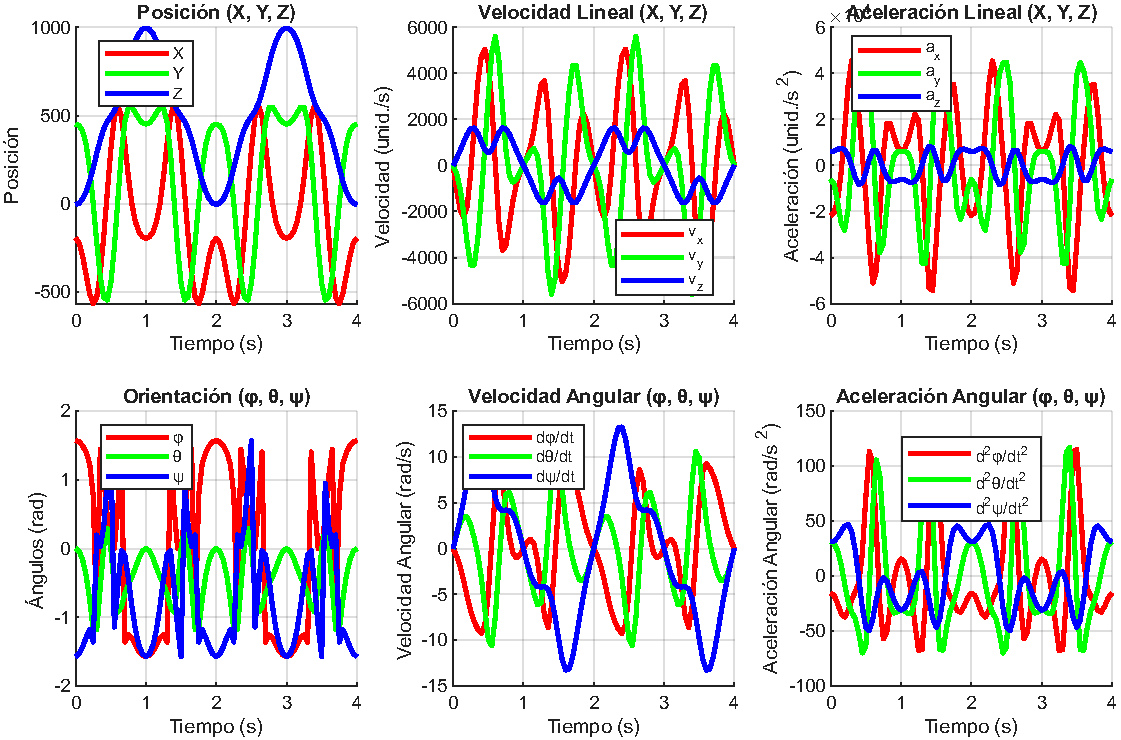
\includegraphics[width=0.8\textwidth]{Graficas_directa_robot_final.pdf}
	\caption{Gráficas cinemática directa en MATLAB.}
	\label{fig:TablasCinematicaDirecta}
\end{figure}

 
 El siguiente conjunto de gráficas representa el comportamiento cinemático de un robot, obtenido mediante la \textbf{cinemática directa} empleando los \textbf{parámetros de Denavit-Hartenberg (DH)}. Cada gráfico describe la evolución de diferentes variables en función del tiempo durante una trayectoria simulada.
 
 \begin{enumerate}
 	\item \textbf{Posición (X, Y, Z)} \\
 	\textit{Gráfica superior izquierda}
 	
 	Muestra la trayectoria espacial del extremo del robot en coordenadas cartesianas.
 	
 	El eje $X$ (rojo), $Y$ (verde) y $Z$ (azul) indican cómo varía la posición en cada uno de los tres ejes con el tiempo.
 	
 	\textbf{Interpretación}: el robot sigue una trayectoria oscilatoria en los tres ejes, lo que sugiere un movimiento complejo, posiblemente cíclico o programado con funciones senoidales o polinomiales.
 	
 	\item \textbf{Velocidad Lineal ($V_x$, $V_y$, $V_z$)} \\
 	\textit{Gráfica superior central}
 	
 	Representa la primera derivada temporal de la posición, es decir, cómo cambia la posición respecto al tiempo.
 	
 	Muestra la rapidez con la que el extremo del robot se mueve en cada dirección.
 	
 	\textbf{Interpretación}: se observa un comportamiento oscilatorio, indicando aceleraciones y desaceleraciones constantes. Las diferencias de amplitud entre ejes indican que el movimiento no es uniforme en todas las direcciones.
 	
 	\item \textbf{Aceleración Lineal ($a_x$, $a_y$, $a_z$)} \\
 	\textit{Gráfica superior derecha}
 	
 	Corresponde a la segunda derivada temporal de la posición.
 	
 	Informa sobre los cambios en la velocidad: aceleraciones positivas y negativas.
 	
 	\textbf{Interpretación}: los valores muestran picos bruscos y cambios rápidos, lo que sugiere que el robot experimenta variaciones rápidas en su movimiento, comunes en trayectorias con alta frecuencia de cambio o maniobras precisas.
 	
 	\item \textbf{Orientación ($\phi$, $\theta$, $\psi$)} \\
 	\textit{Gráfica inferior izquierda}
 	
 	Refleja la orientación del extremo del robot, típicamente representada en ángulos de Euler: roll ($\phi$ - rojo), pitch ($\theta$ - verde) y yaw ($\psi$ - azul).
 	
 	\textbf{Interpretación}: las oscilaciones indican que el robot cambia continuamente su orientación mientras sigue la trayectoria. La transición entre ángulos también sugiere rotaciones complejas, lo cual es habitual en brazos robóticos que deben mantener orientación específica.
 	
 	\item \textbf{Velocidad Angular ($\frac{d\phi}{dt}$, $\frac{d\theta}{dt}$, $\frac{d\psi}{dt}$)} \\
 	\textit{Gráfica inferior central}
 	
 	Representa la velocidad a la que cambian los ángulos de orientación.
 	
 	\textbf{Interpretación}: se identifican zonas de alta velocidad angular, lo que puede indicar maniobras de reorientación rápidas del efector final. El comportamiento es no uniforme y dependiente del ángulo específico.
 	
 	\item \textbf{Aceleración Angular ($\frac{d^2\phi}{dt^2}$, $\frac{d^2\theta}{dt^2}$, $\frac{d^2\psi}{dt^2}$)} \\
 	\textit{Gráfica inferior derecha}
 	
 	Es la segunda derivada de los ángulos respecto al tiempo, y describe cómo varía la velocidad angular.
 	
 	\textbf{Interpretación}: existen picos altos de aceleración angular, lo cual puede deberse a cambios bruscos de orientación en la trayectoria. Estos datos son importantes para evaluar el estrés dinámico sobre las articulaciones del robot.
 \end{enumerate}
 
	
	% Capítulo 5: Conclusiones
	\chapter{Conclusiones} \label{sec:conclusiones}
	\section{Juancito}
Conclusiones y comentarios de Juancito, explicando los problemas que tuvo y lo que aprendió.
	\section{Iliana}
La materia de Robótica fue, para mí, un camino lleno de retos técnicos y personales. Desde el inicio, me enfrenté a conceptos complejos y herramientas con las que no estaba familiarizada, como utilizar LATEX, lo que generó momentos de frustración. Sin embargo, cada obstáculo se convirtió en una oportunidad para aprender y crecer. El proyecto final fue particularmente desafiante y una experiencia muy completa, ya que implicó enfrentar errores, replantear estrategias y colaborar y apoyarme constantemente con mis compañeros. Fue estresante, sobre todo cuando algo no salía como esperábamos, pero también hubo muchos aprendizajes. Aprendí a tener más paciencia, a confiar en el proceso y a no rendirme cuando algo no funcionaba a la primera, aunque fue  gratificante ver los resultados concretos de nuestro trabajo.Gracias a esta materia, no solo adquirí conocimientos técnicos, sino que también fortalecí mi paciencia, mi capacidad de análisis y mi actitud ante los problemas. Robótica me enseñó que equivocarse también es parte del proceso y que con esfuerzo y dedicación, todo aprendizaje es posible.


	\section{Lupita}
Conclusiones y comentarios de Lupita, explicando los problemas que tuvo y lo que aprendió.
	\section{Pepito}
Conclusiones y comentarios de Pepito, explicando los problemas que tuvo y lo que aprendió.
		
	\titleformat{\chapter}
	{\bfseries\huge}
	{}
	{0pt}
	{~\raisebox{-1.5pt}{}
		\\\vspace{.05cm}\titlerule\\\filcenter #1 \\\vspace{.25cm}\titlerule}
	%{\titlerule\\\vspace{.25cm}\filcenter #1 \\\vspace{.25cm}\titlerule}
	\bibliographystyle{IEEEtranN}
	\newpage\label{bibliografia}
	\addcontentsline{toc}{chapter}{Bibliografía}
	
	% Pulsa Ctrl + Clic Izquierdo en bibliografia para entrar.
	\bibliography{bibliografia}
\end{document}


